\documentclass[12pt]{article}
\usepackage[english]{babel}
\usepackage[utf8x]{inputenc}
\usepackage[T1]{fontenc}
\usepackage{scribe}
\usepackage{listings}
\usepackage[version=4]{mhchem}
\usepackage[ISO]{diffcoeff}

\Scribe{Group 17 and Group 18}
\Lecturer{Abir De}
\LectureNumber{9}
\LectureDate{4th september, 2022}
\LectureTitle{Convexity, Trainability and Stability}

\lstset{style=mystyle}

\begin{document}
	\MakeScribeTop

%#############################################################
%#############################################################
%#############################################################
%#############################################################
%%%%% PART 1 %%%%%%%%%%%%%%%%%%%%%%%%%%%%%%%%%%%%%%%%%%%%%%%%%%%%%%%%%%

\section{Definitions}

\subsection{Trainability}

We define trainabilty in order to emphasize on uses of regularization. Being said that, this has not been directly discussed in class. Trainable loss functions requires us to get a bound on expected value of test loss on any test data derived from same distribution as of train data.\par
\hfill \break
\noindent Let A be the algorithm, trained on set S(which is and i.i.d from a distribution P), D denotes the test set derived from same distribution.
\hfill \break
For all $D,\epsilon>0$ there exists $M$ such that for all $m>M$, the following condition holds true
\begin{alignat*}{4}
\underset{s\in P^m}{E}[L_{D}(A(s))] \leq \min_{w}L_{D}(w) + \epsilon 
\end{alignat*}
\subsection{Stability}
Stability is a measure of how the algorithm responds on adding a new data point to the training set. Idea is that we should not give excessive priority to a single data point, more importantly in the cases where the algorithm has already been trained on enough points. This property is also closely related to over-fitting(generating a complex model which reduces loss on train-data, but not on test-data) on data. In some cases stability is also viewed in the terms of drift in model if one of the points is tampered at random. We are going to consider the following metric to view stability.

\begin{alignat*}{4}
\| A(S \cup x) - A(S) \| \; \;where \;
S \in D^m , x \in D\\
\end{alignat*}

We aim at showing that this quantity is bounded and the bound becomes tighter on increasing m tending to 0 for large values of m. 
\noindent and we can increasingly tightly bound this value on expectation.\\
\\
It is not entirely true that more stable  algorithms are better than the less stable ones, consider constant output algorithms for example. A useful algorithm should find a hypothesis that on one hand fits the training set and on the other hand does not over-fit (low structural risk)
\newpage
\subsection{Useful properties of loss functions}
There are lot of properties that a loss function can satisfy which can probably boost performance of algorithm depending on problem requirements.
The following properties are found in most loss functions and are going to be used in the proof that comes up in the next section.

\subsubsection{Convexity}
Convexity of a function helps us to reach its minimum using gradient descent. Convexity of differentiable functions from $R \mapsto R$ is defined by using double derivatives whereas for functions from $R^d$, we define using eigen-values of $\frac{\partial^2 f}{\partial w^2}$.\\
\hfill \break
Condition for a function to be convex given $\frac{\partial^2 f}{\partial w^2}$ exits is that its eigen-values must be non-negative.\\

%Condition for a function to be convex given $\frac{\partial^2 f}{\partial %w^2}$ exits is that its eigen-values must be non-negative, i.e
%$\frac{\partial^2 f}{\partial w^2}$ \text{ should have all non-negative %eigen values}$
\noindent\fbox{
    \parbox{\textwidth}{
        \textbf{Que:- }Find all eigen values of $XX^T, \; X \in m \times1$\\
\textbf{Solution:- }\\
$Rank(XX^T) \leq Rank(X) \leq 1$\\
$Rank(XX^T) \leq 1$\\
$XX^T\; has\; all \;real \; eigen \; values \geq 0$\\
\{$|| x ||^2$, 0 \{with geometric multiplicity m-1\}\} (observe that sum of eigen-values is $\| x \|^2$)\\
    }
}
\subsubsection{Lipschitzness}
Let $C \in R^d$, A function $f: R^d \rightarrow R^k$ is p-Lipschitz over C if for every $w_1, w_2 \in C$ we have \begin{center}$\|f(w_1)-f(w_2)\| \leq p||w_1-w_2||$.\end{center}
Note that Lipschitzness does not guarantee differentiability but differentiable function with bounded derivative is Lipschitz.

\subsubsection{Smoothness}
A differentiable function is $\beta$ - smooth if its gradient is $\beta$ lipschitz.
\begin{alignat*}{4}
    \nabla f(w) = (\frac{\partial f(w)}{\partial w_1}, ..., \frac{\partial f(w)}{\partial w_m})\\
    \|\nabla f(v) - \nabla f(w)\| \leq \beta \|v-w\| 
\end{alignat*}

\noindent\fbox{
    \parbox{\textwidth}{
        \textbf{Note}:
        It can be proven that if f is $\beta$-smooth, following condition holds
        \begin{align*}
            f(v) \leq f(w) + \langle\nabla f(w),v-w\rangle + \frac{\beta}{2} \|v-w\|^2            
        \end{align*}

    }
}



\section{Convexity of Loss Function}
We are given a dataset\\
$$D=\{(x_i,y_i)\}_{i\in[N]} $$
and we are trying to find a model such that
$$\ce{X ->[W] Y}$$
$${w^T}x\approx{y}$$
If we change $x$ by some value, how much $W$ changes.\\
If loss function is convex, perturbation in $W$ is also small.\\
$$l(w^T,x,y)\rightarrow{convex}$$

Examples of convex functions
\begin{itemize}
    \item $\sum{(y-{w^T}x)}^2$
    \item $max(0,1-y{w^T}x)$
    \item $-log(1+{e^{-{w^T}x}})$
\end{itemize}



Example of Non-convex
\begin{itemize}
    \item $(y-({w^T}x)^2+({w^T}x)^3)^2$ is not convex $w.r.t.$ $w$\\
\end{itemize}

Deep learning systems have nice tools that finds local minimum of to search for local minima.\\
Convexity is the requirement of single minima i.e. local minima is the global minima.\\
If loss function is $l(w^T,x,y)$\\

$$\diff*{(l(w^T,x,y))}w \in {\mathbb{R}}^{d\times1}$$ is a vector\\
$$\diff*[2]{(l(w^T,x,y))}{w}\in {\mathbb{R}}^{d\times{d}}$$ is a \textbf{Hessian} matrix.  We require that all its $eigen-values \geq 0$ for $l(w^T,x,y)$ to be convex . \\
For example\\
\textbf{example 1}\\
$l(w)=\sum{(y-{w^T}x)}^2$\\
$${\diff*{(l)}w}=\sum{2(y-{w^T}x)w}$$ 
$$\diff*[2]{(l)}{w}=2XX^T$$ whose eigenvalues are positive (non negative)\\
\\
\textbf{Note } $\diff*[2]{({w^T}Aw)}{w}=A$\\
$XX^T$ is a rank 1 matrix which implies it has one non zero eigenvalue\\
Now, $trace(XX^T) =$ sum of eigenvalues$\rightarrow{}$eigen values are $\{{||x||}^2,0,0 ...\}$\\
Hence, $l(w)=\sum{(y-{w^T}x)}^2$ is a convex function.
\\
\textbf{example 2} \\
$l(w)=max(0,1-y{w^T}x)$\\
It is the maximum of a convex function so it is a convex function.\\
Or, $\frac{\partial^2 {}}{\partial w^2}$ is zero at almost all points, almost everywhere the $eigen-values$ are zero.\\
\\
The plot of $max(0,1-a)$  where $a=y{w^T}x$\\
\begin{center}
    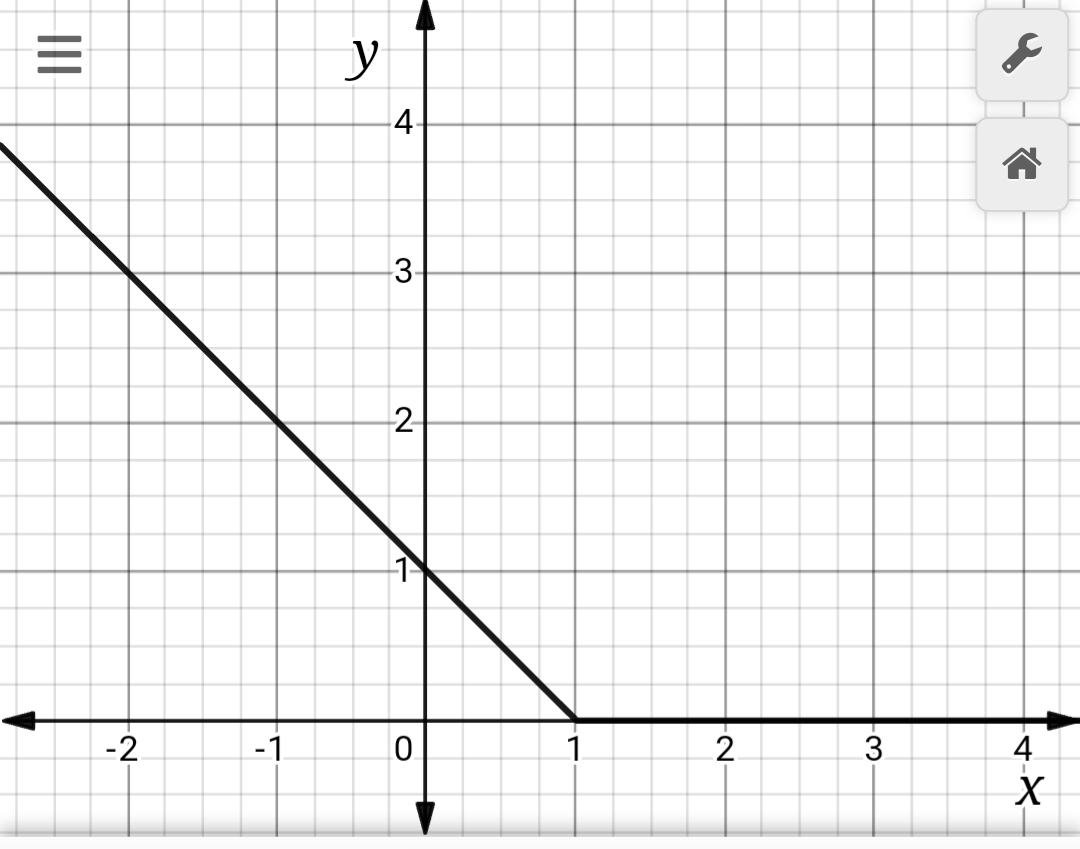
\includegraphics[scale=0.25]{graph.jpg}
\end{center}

%%%%% PART 2 %%%%%%%%%%%%%%%%%%%%%%%%%%%%%%%%%%%%%%%%%%%%%%%%%%%%%%%%%%%%%

\section{Regularization and Stability}
\subsection{Definition}
Most RLM algorithms are in the form given below. We have two terms, one defining fitting of model to given examples and the other representing complexity of the model. 
\begin{alignat*}{4}
   \arg \min_{w}  \;  L_{s}(w) + R(w)
\end{alignat*}
In most scenarios, regularization is used as a tool to reduce over-fitting and provide stability, more on which will be discussed in the section named Regularisation and Stability.
\subsection{Uses}
There are many uses of introducing regularization but most prominent ones are the following :
\begin{itemize}
\item Balance between fitting and stability
\item Only some of the functions in the convex smooth domain can be proved to be trainable. But with correct regularization, all smooth convex functions can be shown to be trainable.
\end{itemize}
Hence, RLM can be used as a general learning rule for convex smooth learning problems.\\
You may have already intuitively noticed this in previous classes where $XX^{T}+$ $\lambda$I ($\lambda>0$)  is shown to always have an inverse  .\\
\\
Tikhonov Regularization : \indent
$R(w) := \lambda \| w \|^{2} $
\\
Adding regularizer terms leads to a \textbf{strictly convex} loss function.
$$l_{\lambda}(w,x,y) = \sum{(y-{w^T}x)}^2 +\lambda||w||^2 $$
$$l_{\lambda}(w,x,y) = l(w,x,y) +\lambda||w||^2 $$

\subsection{Assumptions regarding loss function}
\begin{enumerate}
    \item $l_{\lambda}(w,x,y) = l(w,x,y) +\lambda||w||^2 $ is strictly convex, since $\diff*[2]{(l_{\lambda}(w,x,y))}{w} > 0$
    \item  $\normx{\diff{l(w,x,y)}{w}}$ is \textbf{bounded} , i.e $\normx{\diff{l(w,x,y)}{w}} \leq $ B
    \item $\normx{W(D U K) - W(D)} = \mathcal{O}(\frac{1}{|D|})$
\end{enumerate}
\noindent
Let's prove the assumptions,
$$\diff*[2]{(l_{\lambda}(w,x,y))}{w}= \diff*[2]{(l(w,x,y))}{w} + 2\lambda \mathbb{I}$$ 
whose eigenvalues are \textbf{strictly} \textbf{positive}. Since $\lambda>0$, $2\lambda\mathbb{I}$ has strictly positive eigenvalues, while  $l(w,x,y)$ has non negative eigenvalue as shown earlier. Hence $l_{\lambda}(w,x,y))$ is strictly convex.\\

%%%%% PART 3 %%%%%%%%%%%%%%%%%%%%%%%%%%%%%%%%%%%%%%%%%%%%%%%%%%%%%%%%%

$$F(W,S) = \sum_{i = 1}^{|S|} l_{\lam}(W,x_i,y_i)$$
$$W(S) = \underset{W}{min}\sum_{i = 1}^{|S|} l_{\lam}(W,x_i,y_i)$$
 First of all , note that $F(W(S \cup K),S) - F(W(S),S)$ > 0 because W(S) is the value of W that minimizes F(W,S) . \\ 
We want to bound $F(W(S \cup K),S) - F(W(S),S)$. A simple bound on this difference using the notion of Lipschitz continuity is
$$ F(W(S \cup K),S) - F(W(S),S) \leq B_{\lam}|S| \normx{W(S \cup K) - W(S)}$$
Now we attempt to form a tighter bound on $F(W(S \cup K),S) - F(W(S),S)$ \\
We can split $F(W(S),S)$ as $F(W(S),S \cup K) - F(W(S),K)$
\noindent
Note that K is a single data point .
 \begin{align*}
     F(W(S \cup K),S) - F(W(S),S) &= (F(W(S \cup K),S \cup K) - F(W(S),S \cup K)) \\
     & + (F(W(S),K) - F(W(S \cup K),K)) 
 \end{align*}
\noindent
$F(W(S \cup K),S \cup K) - F(W(S),S \cup K) \leq 0 $ because $W(S \cup K)$ is the optimal value of W which minimizes $F(W,S \cup K)$ .\\
F is Lipschitz continuous . Hence ,
\begin{align*}
    F(W(S),K) - F(W(S \cup K),K)  &= (W(S) - W(S \cup K))^T\frac{\partial F}{\partial W}\bigg|_{W'} \\
    & \leq B\normx{W(S \cup K) - W(S)}
\end{align*}
Here we used the Assumption 2 regarding loss function that the first derivative is bounded by some constant B .
\noindent
Hence , we proved that 
\begin{equation}
    \label{ineq1}
    F(W(S \cup K),S) - F(W(S),S) \leq B\normx{W(S \cup K) - W(S)}
\end{equation}

Now we try to find a lower bound for the expression $F(W(S \cup K),S) - F(W(S),S)$ using the convexity of the loss function .

First we apply Taylor Series Expansion to $F(W(S \cup K),S)$
\begin{align}
    F(W(S \cup K),S)  &=  F(W(S),S) + (W(S \cup K) - W(S))^T\frac{\partial F}{\partial W}\bigg|_{W = W(S)} \nonumber \\
    & + \frac{1}{2!}(W(S \cup K) - W(S))^T H(W)(W(S \cup K) - W(S)) \nonumber \\
    &= F(W(S),S)  + \frac{1}{2}(W(S \cup K) - W(S))^T H(W)(W(S \cup K) - W(S))
    \label{ineq}
\end{align}
Where $H(W) = \frac{\partial^2 F}{\partial^2 W}$ is the Hessian Matrix  corresponding to F at some $W^*$ lying on the line between W(S) and $W(S \cup K)$.
Here we used the idea that $\frac{\partial F}{\partial W}|_{W = W(S)} = 0$ because W(S) is the optimum value which minimizes F(W,S)

Note from Assumption 1 we have that all eigen values of the double derivative of $l(w,x,y)$(loss function with regularization) w.r.t. W  are positive. In other words , all eigen values of $\frac{\partial^2 l(W,x,y)}{\partial^2 W}$ are positive .  
\begin{align}
    F(W,S) &=  \sum_{i = 1}^{|S|} l_{\lam}(W,x_i,y_i) \nonumber\\
          &=  \sum_{i = 1}^{|S|}l(W,x_i,y_i) + \sum_{i = 1}^{|S|} \lam \normx{W}^2  = \sum_{i = 1}^{|S|}l(W,x_i,y_i) + \lam|S|\normx{W}^2\nonumber
\end{align}
\begin{align}
    H(W)   &=  \frac{\partial^2 F(W,S)}{\partial^2 W} \nonumber\\
           &=  \frac{\partial^2 \sum_{i = 1}^{|S|} l_{\lam}(W,x_i,y_i)}{\partial^2 W}\nonumber\\
           &=  \sum_{i = 1}^{|S|} \frac{\partial^2 l(W,x_i,y_i)}{\partial^2 W} + 2\lam |S| I\nonumber\\
   v^TH(W)v &=  \sum_{i = 1}^{|S|} v^T\frac{\partial^2 l(W,x_i,y_i)}{\partial^2 W}v + 2\lam |S| v^Tv\nonumber\\
         & \geq 2\lam |S|\normx{v}^2 \nonumber
\end{align}
Apply this to \eqref{ineq} , we get 
\begin{equation}
    \label{ineq2}
    F(W(S \cup K),S) - F(W(S),S) \geq ||W(S \cup K) - W(S)||^2 \lam |S|
\end{equation}
From \ref{ineq1} and \ref{ineq2} , we have 
\begin{align*}
    ||W(S \cup K) - W(S)||^2 \lam |S| &\leq F(W(S \cup K),S) - F(W(S),S) \leq B\normx{W(S \cup K) - W(S)} 
\end{align*}
\begin{align*}
    ||W(S \cup K) - W(S)||^2 \lam |S| &\leq  B\normx{W(S \cup K) - W(S)} \\
    ||W(S \cup K) - W(S)||  &\leq \frac{B}{\lam |S|}
\end{align*}
Thus we have proved Assumption 3 which states that  
\begin{equation}
    \normx{W(S \cup K) - W(S)}  = \calO(\frac{1}{|S|})
\end{equation}


\subsection{Regularization and Stability}
Stability, as defined earlier is measured by the quantity
\[
    \|A(S \cup x)-A(S)\| 
\]
where x is new data point added to S.\\
proving the stability requires us to prove that$\underset{S \in D^m}{\|}A(S \cup x)-A(S)\|$ is bounded and the bound becomes tighter as m increases, converging to 0. We prove this result considering bounds of 
\[
    E=L(A,S(A \cup x)) - L(A,S(A))
\]
Note that this quantity is greater than 0 for a good algorithm and loss function i.e $E>0$.
\vspace{-10pt}
\subsubsection{Proving upper bound}
\indent Using the Smoothness/ lipschitz
\[L(A,S(A \cup x)) - L(A,S(A)) < B(m) ||S(A \cup m)- S(A)||\]
This sure is a bound but not a good one as the factor m destroys the purpose of the bound, which will be clear by the end of this proof .
\begin{gather}
    L(A,S(A \cup x)) - L(A,S(A)) = L(A \cup x, S(A \cup x)) - L(x, S(A \cup x)) - (L(A \cup x,S(A)) - L(x,S(A))) \\
    let \; G(M) = L(A \cup x, S(M))-L(x,S(M))
\end{gather}
Observe that eq 1 can be rewritten as 
\begin{gather}
    G(A\cup x)-G(A)
\end{gather}
using smoothness of eq 3 we can write
\begin{gather}
    G(S(A \cup x)) - G(S(A)) \leq B || S(A \cup x)- S(x) ||
\end{gather}

\subsubsection{Proving lower bound}
\indent This proof uses a non-trivial result from taylor series which will be stated as lemma.\\[7pt]
\noindent\fbox{
    \parbox{\textwidth}{
    \textbf{Lemma-1}:- \\
        \[
            f(h_1) \geq f(h_2) + <\triangledown f(h_1,h_1-h_2)> + \frac{1}{2}(h_1-h_2)^{T} \triangledown^2f(h^{`},h_1-h_2^{`})
        \]
        for some $h^{`}$.
    }
}
\\[9pt]
Apply lemma-1 on eq 1, we get 
\begin{gather}
\begin{split}
    L(A,S(A \cup x))- L(A,S(A)) \geq \; < \triangledown L(A,S(A)), S(A\cup x)- S(A) > \\+ \frac{1}{2}(S(A\cup x)-S(A))(\triangledown^2 l(A,h^{`})*m)(S(A \cup x)-S(A))
\end{split}
\end{gather}
Observe that $\triangledown L(A,S(A))=0$, by definition
\begin{gather}
    L(A,S(A \cup x))-L(A,S(A)) \geq \frac{m}{2} (S(A \cup x)-S(A))^{T} \triangledown^2 l(A,h^{`})(S(A \cup x)-S(A))
\end{gather}
considering the case of Tiknow regularisation $eig(\triangledown^2 L(A,h)) \geq \lambda$ giving \begin{gather}
    L(A,S(A \cup x)) - L(A,S(A)) \geq \frac{m}{2} \lambda || S(A \cup x) - S(A) ||^2
\end{gather}

using Eq 7 and 4
\begin{gather}
    B||S(A \cup x) - S(A)|| \geq \frac{\lambda}{2}\m  ||S(A \cup x)-S(A)||^2\\
    \frac{2B}{\lambda m}\geq ||S(A \cup x )-S(A)||
\end{gather}

\noindent \fbox{
    \parbox{\textwidth}{
        \textbf{Question:-}\\
        On similar lines, derive a bound for following case $||S(A^{`})-S(A)||$ where $A^{`}$ is set with one case ($z_i$) tampered to ($z_i^{`}$).\\[4pt]
        \textbf{HINT}\\
        \[
            ||\overline{S}(A^{`} \cup Z_i) + S(A^{`}) + S(A \cup Z_i^{`}) -S(A) ||= ||S(A^{`})-S(A)||
        \]
    }
}

%% PART 4 %%%%%%%%%%%%%%%%%%%%%%%%%%%%%%%%%%%%%%%%%%%%%%%%%%%%%%%%%%%%%%%%

\section{Non Linear Regression}
In nonlinear regression, we modeled a given data-set by using a function which is a nonlinear combination of the model parameters and depends on one or more independent variables.
\\ That is why nonlinear regression shows association using a curve, making it nonlinear in the parameter.
\\In contrast to linear regression, we cannot use the ordinary least squares method to fit the data and estimation of the parameters are also not easy.
\\
\\Let's think about the solution
\\
\begin{equation}
    w = (\lambda I + \sum\limits_{i\epsilon D} X_i X^T )^{-1} \sum\limits_{i\epsilon D} X_i Y_i
\end{equation}
\\In linear case, we have a line graph. So, what do we have to change in our approach to fit the non-linear regression$?$
\\
\\What is that $X_i X^T$ indicates?
\\
\[
   X_i X^T = ||X_i||^2
\]
\\Suppose we have two vector [1 2 3]$^T$ and [3 6 9]$^T$.
\\Are they similar?
\\Although its directions are same but these are not the similar points.
\\
\\If the given two points are close enough that its covariance is atleast 0.7, then we will consider the data set as comparately similar to linear regression otherwise we have to think of the non-linear regression otherwise we have to think of th non-linear regression.
\\
\\Instead of term $X_i X^T$, we can put the Kernel $K(X_i X_i)$ to get some sort of good approximation to our non-linear data set.
\\
\\ \textbf{Example}
\\ For infinite dimension vector in infinite dimension space :-
\\The measure of \textbf{similarity} between $\vec{X_i}$ and $\vec{Y_i}$ is approximate to
\[
     e^{-||X_i - X_j||^2}
\]
\\Instead of $X_i X^T$, take the matrix formed by using the above equation for each entry (i,j).
\\The above equation $e^{-||X_i - X_j||^2}$ can be represented as the dot product of two vectors.
\\
\\Dot product isn't the good measure of similarity
\\Other measures are:-
\\
\[
     e^{-||X_i - X_j||^2}
\]\[
     \frac{1}{1 + ||X_i - X_j||^2}
\]
\\
\\We can replace $X^TX$ by K in the loss function to get
\\
\begin{equation}
    w = (\lambda I + K)^{-1} \sum\limits_{i\epsilon D} X_i Y_i
\end{equation}
Here, K is the Kernel matrix
\\\[
    e^{-||X_i - X_j||^2} => \phi_i^T \phi_j
\]
\\Doing non-linearity in finite dimension to linearity in infinite dimension space 
\subsection{Stability}
It is easy for linear regression but it is bit difficult for non linear regression.
\\So, we need to apply \textbf{deep learning} for those data 
 sets which don't have linearity even in infinite dimension i.e, $\phi_i^T \phi_j$
 \\
 \\\textbf{Example}
 \[
    \{ \vec{x_i}, y_i | i \epsilon D \}
\]
\\For the above example, linear regression or kernel both didn't work.
\\We can use deep learning concepts to find some relation between data sets i.e, Y = F($\vec{X}$).
\\We can approximate any kind of functions for the given set of data that follows non linearity using functions like ReLU , Sigmoid and Tanh.
\\For example, try to find a linear model for y = log(x) such that x $>$ 0.
\\
\\


%%%%%%%%%%% If you don't have citations then comment the lines below:
%
%\bibliographystyle{abbrv}           % if you need a bibliography
%\bibliography{mybib}                % assuming yours is named mybib.bib


%%%%%%%%%%% end of doc
\end{document}
